\documentclass[tikz]{standalone}%

\usepackage[utf8]{inputenx}%  http://ctan.org/pkg/inputenx
% Euler for math | Palatino for rm | Helvetica for ss | Courier for tt
\renewcommand{\rmdefault}{ppl}% rm
\linespread{1.05}% Palatino needs more leading
\usepackage[scaled]{helvet}% ss //  http://ctan.org/pkg/helvet
\usepackage{courier}% tt // http://ctan.org/pkg/courier
\usepackage{eulervm}  %  http://ctan.org/pkg/eulervm
% a better implementation of the euler package (not in gwTeX)
\normalfont%
\usepackage[T1]{fontenc}%  http://ctan.org/pkg/fontenc
\usepackage{textcomp}%  http://ctan.org/pkg/textcomp

\usetikzlibrary{angles}
\usetikzlibrary{quotes}

%  draws block hanging from a string
\newcommand\block{
  \draw (0, 0) -- (0, -1.5cm) -- (-.5cm, -1.5cm) rectangle (.5cm, -2.5cm);}

\begin{document}
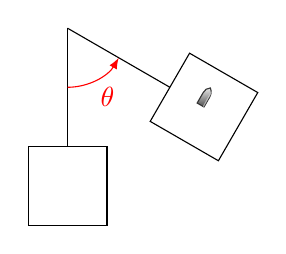
\begin{tikzpicture}
  \coordinate (O) at (0, 0);
  \coordinate (P1) at (0, -1.5cm);
  
  \block

  \begin{scope}[rotate = 60]
    \coordinate (P2) at (0, -1.5cm);
   
    \block
  \end{scope}

  \path (P1) -- (O) -- (P2) pic["$\theta$", draw, -latex, red,
  angle radius = 0.75cm, angle eccentricity = 1.35] {angle = P1--O--P2};

  \coordinate (A) at (-30:2cm);  % To position the bullet in another fig

  \begin{scope}[shift = {(A)}, rotate = 60]
    \fill[draw = black!80, top color = black!10, bottom color = black!70]
    (0, 1mm) -- (1.5mm, 1mm) to [out = 0, in = 120] (2.5mm, 0.5mm) 
    to[out = -120, in = 0] (1.5mm, 0) -- (0, 0) -- cycle;
    \draw[white, draw opacity = 0.5] (0, 0.1mm) -- (2.3mm, 0.1mm);
  \end{scope}
\end{tikzpicture}
\end{document}
%%% Local Variables:
%%% mode: latex
%%% TeX-master: t
%%% End:
